\documentclass[../main/main.tex]{subfiles}

\newdate{date}{13}{12}{2019}


\begin{document}

\marginpar{ \textbf{Lecture 18.} \\  \displaydate{date}. \\ Compiled:  \today.}

\subsection{Solution by Fourier transform}
Let us try to do the Fourier transform and define
\begin{equation}
  \va{x} \equiv \va{r} - \va{r}'
\end{equation}
 Taking the Fourier transform of
\begin{equation}
  \qty(- \grad ^2 + \xi ^{-2} (t)) G_c (\va{r}-\va{r}') = \frac{k_B T}{k} \delta (\va{r}-\va{r}')
\end{equation}
and calling \( \widetilde{G} (q)  \) the Fourier transform of the function \( G \), one gets
\begin{equation}
  \widetilde{G} (q) = \int_{- \infty }^{+ \infty } \dd[]{\abs{\va{x}} } G_c ( \abs{\va{x}} ) e^{- i q \abs{\va{x}} } \quad
   \Rightarrow \widetilde{G} ( q ) = \frac{k_B T}{k} \frac{1}{q^2 + \xi ^{-2}}
\end{equation}
\begin{remark}
At \( T = T_c \), since  \( \xi \rightarrow \infty  \)  we have  and \( \widetilde{G} (q) \simeq \frac{1}{q^2}  \) and performing the inverse Fourier transform one gets
\begin{equation}
  G_c (\abs{\va{x}} ) = \abs{\va{x}}^{2-D}
\end{equation}
On the other hand, at \( T=T_c \) we defined
\begin{equation}
  G (r) \sim \abs{\va{x}}^{2-D- \eta }
\end{equation}
hence, we have \( \eta =0 \).
\end{remark}
Let us now obtain the full expression of \( G(r) \) by computing the inverse Fourier transform
\begin{equation}
  G (\va{x}) = \int_{}^{} \dd[D]{\va{q}}  \frac{1}{(2 \pi )^D} \frac{1}{q^2 + \xi ^{-2}} e^{i \va{q} \vdot \va{x}}
\end{equation}
Let us do it for \( D=3 \):
\begin{equation}
\begin{split}
G(\va{x})  &=  \int_{}^{} \dd[3]{\va{q}}  \frac{1}{(2 \pi )^3} \frac{1}{q^2 + \xi ^{-2}} e^{i \va{q} \vdot \va{x}} \overset{\substack{ \text{spherical} \\ \text{coordinates}} }{=}  \\
& = \frac{4 \pi }{ (2 \pi )^3} \int_{0}^{\infty } \dd[]{q} \frac{q^2}{q^2+ \xi ^{-2}} \int_{-1}^{+1} \dd[]{(\cos \theta  )}    e^{i q \abs{\va{x}} \cos \theta  } \\
& \overset{z \equiv \cos(\theta ) }{=} \frac{2}{(2 \pi )^2} \int_{0}^{\infty } \dd[]{q} \frac{q^2}{q^2 + \xi ^{-2}} \qty[\frac{1}{i q \abs{\va{x}} } e^{i q \abs{\va{x}} z } ]_{-1}^{1}   \\
& = \frac{4}{(2 \pi )^2 \abs{\va{x}} } \int_{0}^{\infty } \frac{q \sin(q \abs{\va{x}} ) }{q^2 + \xi ^{-2}} \dd[]{q}
\end{split}
\end{equation}
Let us now consider the integral
\begin{equation}
  I = \int_{0}^{\infty } \frac{q \sin(q \abs{\va{x}} ) }{q^2 + \xi ^{-2}} \dd[]{q}
  = \frac{1}{2} \int_{- \infty }^{+ \infty } \frac{q \sin(q \abs{\va{x}} ) }{q^2 + \xi ^{-2}} \dd[]{q}
\end{equation}
that can be computed in the complex plane, i.e. as
\begin{equation}
  I = \frac{1}{2} \Im \oint \frac{z e^{i z \abs{\va{x}} } }{\qty(z^2 + \xi ^{-2}) } \dd[]{z}
\end{equation}
The integration contour is a semicirle in the positive half plane. There are two poles \( z_P = \pm i \xi ^{-1} \), but only one is enclosed by the semicirle (Figure \ref{fig:18_1}).

\begin{figure}[h!]
\centering
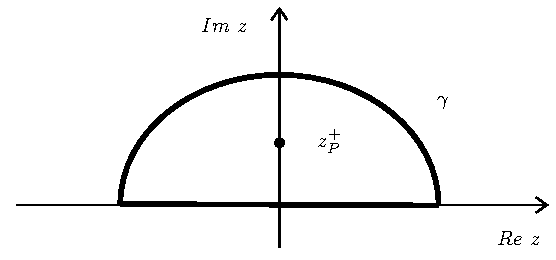
\includegraphics[width=0.6\textwidth]{../lessons/18_image/1.pdf}
\caption{\label{fig:18_1} Description.}
\end{figure}

Using the Theorem of residues one has
\begin{equation}
\begin{split}
I  &=  \frac{1}{2} \Im \oint_\gamma \frac{z e^{i z \abs{\va{x}} } }{\qty(z^2 + \xi ^{-2}) } \dd[]{z} = \frac{1}{2}  \oint_\gamma \frac{z e^{i z \abs{\va{x}} } }{ \qty(z + i \xi ^{-1}) \qty(z - i \xi ^{-1})  } \dd[]{z}  \\
& \overset{th.\, of\, residues}{=}  \frac{1}{2} \Im \qty[2 \pi  i \text{Res} (i \xi ^{-1})]
\end{split}
\end{equation}
and since
\begin{equation}
  \text{Res} (i \xi ^{-1}) = \frac{i \xi ^{-1} e^{- \xi ^{-1} \abs{\va{x}} } }{2 i \xi ^{-1}} = \frac{e^{-\abs{\va{x}}/\xi  } }{2}
\end{equation}
\begin{equation}
  \Rightarrow  I = \frac{1}{2} \Im \qty[2 \pi  i \text{Res} (i \xi ^{-1})] = \frac{\pi }{2} e^{- \abs{\va{x}} /\xi }
\end{equation}
Hence, at the end
\begin{equation}
  \Rightarrow G ( \abs{\va{x}} ) = \frac{1}{2 \pi } \frac{e^{- \frac{\abs{\va{x}} }{\xi }} }{\abs{\va{x}} }
\end{equation}
where it is confirmed the exponential behaviour for \( t \neq 0 \) and \( \eta =0 \).

One can also solve the equation for \( G(\va{r}- \va{r}') \)   by using the spherical coordinates and use the Bessel functions.


\section{Including fluctuations at the Gaussian level (non interacting fields)}
Can we reach the simple level of fluctuation? The simple level is the one that follow gaussian distribution.
Let us introduce fluctuations at the Gaussian level.

Let us consider \( h=0 \) and let \( m_0 (\va{r})= m_0 \) be the solution of the saddle point approximation. Let us expand the general expression
\begin{equation}
  \beta \mathcal{H}_{eff}  [m] = \int_{}^{} \dd[D]{\va{r}} \qty( a t m^2 + \frac{b}{2} m^4 + \frac{k}{2} \qty(\grad m)^2 )
\end{equation}
by using
\begin{equation}
  m(\va{r}) = m_0 + \delta m(\va{r})
\end{equation}
We are assuming that the fluctuations \(  \delta m(\va{r})\) are small:
\begin{subequations}
\begin{align}
   \qty(\grad m)^2 &= \qty(\grad \qty(m_0 + \delta m) )^2 = \qty(\grad \qty(\delta m) )^2  \\
     m^2 &= m_0^2 + 2 m_0 \delta m + \qty(\delta m)^2 \\
     m^4 &= m_0^4 + 4 m_0^3 \delta m + 6 m_0^2 (\delta m)^2 + 4 m_0 \delta m^3 + (\delta m)^4
\end{align}
\end{subequations}
Hence,
\begin{equation}
  \beta \mathcal{H}_{eff} = V \underbrace{ \qty(a t m_0^2 + \frac{b}{2} m_0^4) }_{A_0}
  + \int_{}^{} \dd[D]{\va{r}} \qty(\frac{k}{2}\qty(\grad m)^2 + \qty(a t + 3 b m_0^2)\delta  m^2 + 2 b m_0 \delta m^3 + \frac{b}{2} \delta m^4 )
\end{equation}
\begin{remark}
The term proportional to \( \delta m \),  \( \qty( 2 a t m_0  + \frac{b}{2} 4 m_0^3 )  \) is zero since \( m_0 \) is the solution of the extremal condition
\begin{equation}
  \eval{\frac{\delta \mathcal{H}_{eff}}{\delta m}}_{m=m_0} = 0
\end{equation}
\end{remark}

For simplicity let us first consider \( T>T_c \),  we know that \( m_0 = 0 \) and
\( m (\va{r}) = m_0 + \delta m(\va{r}) = \delta m (\va{r}) \). We have \( A_0 =0 \), \( 3bm_0^2 \delta m^2 = 0 \) and \( 2 b m_0 \delta m^3 = 0 \), that implies
\begin{equation}
  \beta \mathcal{H}_{eff}^{T>T_c} (\delta m)= \int_{}^{} \dd[D]{\va{r}} \qty(\frac{k}{2} \qty(\grad \delta m)^2 + a t (\delta m)^2 + \cancel{\frac{b}{2} (\delta m)^4} )
\end{equation}
\begin{remark}
It is important to understand that these are fluctuations with respect to the solution.
\end{remark}
The Gaussian approximation consists in neglecting the quartic term \( (\delta m)^4 \)
\begin{equation}
  \Rightarrow
    \beta \mathcal{H}_{eff}^{T>T_c} (\delta m) \simeq  \int_{}^{} \dd[D]{\va{r}} \qty(\frac{k}{2} \qty(\grad \delta m)^2 + a t (\delta m)^2 )
\end{equation}

\section{lesson}


We cannot do again the saddle point, otherwise we do not get too much information.
We consider gaussian fluctuations: fluctuations that follow gaussian distribution.
Therefore, the term in \( (\delta m)^4 \)  is cancelled.
What it is the difference in the exponent respect the mean field?
Then we will to the same for \( T < T_c \), the story is the same. Now, we are just taking the gaussian term
\begin{equation}
  Z_{GL}^G = \int_{}^{} \text{D} \qty[\delta m] e^{- \int_{}^{} \dd[D]{r} \qty(\frac{k}{2} \qty(\grad \delta m)^2 + a t (\delta m)^2  )  }
 \end{equation}
Consider a system in a box of volume \( V = L^D \):
\begin{equation}
  \delta m (\va{r}) = \frac{1}{V} \sum_{}^{\va{k}}  e^{i \va{k}\vdot \va{r}} \delta m_{\va{k}}
\end{equation}
We have the integral
\begin{equation}
  \delta m_{\va{k}} = \int_{V}^{} \dd[D]{\va{r}} \delta m (\va{r}) e^{-i \va{k} \vdot \va{r} }
\end{equation}
with \( \va{k} = k_1, \dots, k_D = \frac{2 \pi  \bar{n} }{L}\)
We have \( \delta m_{\va{k}} \in \mathbb{C} \) but \( \delta m (\va{r}) \in \R \), hence
\begin{equation}
  \delta m_{\va{k}} = - \delta m_{-\va{k}}
\end{equation}
\begin{equation}
  \sum_{\va{k}}^{} \rightarrow \frac{V}{( 2 \pi )^D} \int_{\R}^{} \dd[]{\va{k}}
\end{equation}
\begin{equation}
  \frac{1}{V} \sum_{\va{k}}^{} e^{i \va{k} (\va{r}-\va{r}')} \rightarrow \frac{1}{V} \frac{V}{(2 \pi )^2} \int_{\R}^{} \dd[D]{\va{k}} e^{i \va{k} (\va{r}-\va{r}')}
  = \delta (\va{r}- \va{r}')
\end{equation}
\begin{equation}
  \frac{1}{V} \int_{}^{} \dd[D]{\va{r}} e^{i (\va{k} - \va{k}') \vdot  \va{r}} = \delta _{\va{k}\va{k}'}
\end{equation}
write immediately
\begin{equation}
  V \delta _{\va{k} \va{k}'} \overset{V \rightarrow \infty }{\longrightarrow  } (2 \pi )^D \delta (\va{k} - \va{k}')
\end{equation}
\begin{equation}
  a \Rightarrow \abs{\va{k}} \le \frac{\pi }{a} = \Lambda
\end{equation}
that is the ultraviolet cut-off.

Change now the notation:
\begin{equation}
  \delta m (\va{r}) \leftrightarrow \varphi (\va{r}), \quad k \leftrightarrow c
\end{equation}
and obtain
\begin{equation}
  \beta \mathcal{H}_{eff}^{G,>} = \int_{}^{} \dd[D]{\va{r}} \qty[\frac{c}{2} \qty(\grad \phi )^2 + a t \phi ^2 ]
\end{equation}
\begin{equation}
\begin{split}
  \int_{}^{} \dd[D]{r} \frac{c}{2} \qty(\grad \varphi )^2 & = \frac{c}{2} \frac{1}{V^2} \int_{}^{} \dd[D]{\va{r}} \qty(\grad \sum_{\va{k}}^{} e^{i \va{k} \vdot \va{r}} \varphi _{\va{k}}  ) \qty(\grad \sum_{\va{k}'}^{} e^{i \va{k}' \vdot \va{r} } \varphi _{\va{k}'}  )     \\
  & = \frac{c}{2} \sum_{\va{k} \va{k}'}^{}  \qty(- \va{k} \va{k}') \varphi _{\va{k}} \varphi _{\va{k}'} \underbrace{\int_{}^{} \dd[D]{\va{r}}  e^{i (\va{k}+\va{k}')\vdot \va{r}}}_{(2 \pi )^2 \delta (\va{k}+ \va{k}')}   \\
  & = \frac{c}{2V} \sum_{\va{k}}^{} \abs{\va{k}}^2 \varphi _{\va{k}} \varphi _{\va{-k}'}
\end{split}
\end{equation}
\begin{equation}
  \beta \mathcal{H}_{eff}^{G,>} \rightarrow \frac{1}{2V} \sum_{\va{k}}^{} \qty(2 a t + c k^2) \varphi _{\va{k}} \varphi _{-\va{k}'}
\end{equation}
\begin{equation}
  \int_{}^{} \text{D} \qty[\varphi (\va{r})] \rightarrow \int_{- \infty }^{+ \infty } \prod_{\abs{\va{k}} < \Lambda  }^{}   \dd[]{(\Re{\varphi _{\va{k}}})}   \dd[]{(\Im{\varphi _{\va{k}}})}
\end{equation}
with \( \varphi _{\va{k}} \in \mathbb{C} \).
\begin{equation}
  \varphi _{\va{k}}^* = \varphi _{-\va{k}}
\end{equation}
\begin{equation}
  \Re {\varphi _[\va{k}]} = \Re {\varphi _{-\va{k}}}, \quad   \Im{\varphi _[\va{k}]} = -\Im {\varphi _{-\va{k}}}
\end{equation}
\begin{equation}
  \Tr = \int_{- \infty }^{+ \infty } \prod_{\substack{ \abs{\va{k}} < \Lambda   \\ k_D > 0 } }^{}   \dd[]{\Re {\varphi _{\va{k}}}}  \dd[]{\Im {\varphi _{\va{k}}}}
\end{equation}
\begin{equation}
  \widetilde{Z}_{GC}^{G,>} = \frac{1}{2} \int_{- \infty }^{+ \infty } \prod_{\substack{ \va{k}   \\\abs{\va{k}} < \Lambda } }^{} \dd[]{\Re {\varphi _{\va{k}}}}  \dd[]{\Im {\varphi _{\va{k}}}}
  e^{- \beta \widetilde{\mathcal{H}}_{eff} [\varphi _{\va{k}}] }
\end{equation}
\begin{equation}
  x = \Re \varphi _{\va{k}}, \quad   y = \Im \varphi _{\va{k}}
\end{equation}
\begin{equation}
  \int_{-\infty }^{+\infty } \dd[]{x} \dd[]{y} e^{-A (x^2+y^2)} = \frac{\pi }{A}
\end{equation}
where \( A= \frac{1}{2V} \).
\begin{equation}
  e^{-\beta \widetilde{F}_{GL}^> } = \qty(\prod_{\substack{\va{k} \\ \abs{\va{k}} <\Lambda \\ k_D > 0  } }^{}  \frac{2 \pi V}{2 a t + c \abs{\va{k}}^2 } )
\end{equation}
\begin{equation}
  \widetilde{F}_{GL}^{G,>} = - \frac{1}{2} k_B T \sum_{\abs{\va{k}}> \Lambda  }^{}
  \log{\qty(\frac{2 \pi V}{2 a t + c \abs{\va{k}}^2 })}
\end{equation}
\begin{equation}
  c_V = - T \pdv[2]{F}{T} = \frac{A}{V} \sum_{\abs{\va{k}} < \Lambda  }^{}
  \frac{1}{2 a t + c \abs{\va{k}}^2 } - \frac{B}{V} \sum_{\abs{\va{k}}< \Lambda  }^{} \frac{1}{\qty(2 a t + c \abs{\va{k}}^2)^2 }
\end{equation}
Question: what happens if I introduce guassian fluctuations.

It turns out that when we study the asimptotic behaviour of these integrals.

For the first term it turns out that
\begin{equation}
1^{st} \propto
  \begin{cases}
   \xi ^{4-D} \sim t^{-\nu (4-D)}  & D < 4\\
  < \infty & D > 4
  \end{cases}
\end{equation}
\begin{equation}
2^{nd} \propto
  \begin{cases}
   \xi ^{2-D} \sim t^{-\nu (2-D)}  & D < 2\\
  < \infty & D > 2
  \end{cases}
\end{equation}
At the end, the behaviour of the specific heat
\begin{equation}
  c_V \sim \begin{cases}
    t^{-\nu (4-D)} & D < 4 \\
    \infty & D > 4
\end{cases}
\end{equation}
figure 1, figure 2.
\begin{equation}
  \expval{\varphi _{\va{k}} \varphi _{\va{k}'}}_G = \frac{\int_{}^{} \prod_{}^{}   \dd[]{\varphi _{\va{k}}}  \dots e^{- \beta \mathcal{H}_{eff}}  \phi_{\va{k}} \varphi _{\va{k}'} }{Z_{GL}^{G,>}}
  = \delta _{\va{k},\va{k}'} \frac{V}{2 a t + c k^2}
\end{equation}
\begin{equation}
\Rightarrow
  \begin{cases}
   \nu _G = \frac{1}{2}\\
   \eta_G = 0
  \end{cases}
\end{equation}









\end{document}
